\documentclass[letterpaper, 11pt]{article}
\usepackage{latexsym}
\usepackage{amssymb}
\usepackage{times}
%\usepackage[in]{fullpage}
\usepackage{amsmath,amsfonts,amsthm}
\usepackage{graphicx}

%\documentclass[11pt]{article}
%\pagestyle{myheadings}
%\usepackage[ruled,nothing]{algorithm}
%\usepackage{algorithmic}
%\usepackage[dvips]{epsfig,graphicx}
%\numberwithin{equation}{section}

\bibliographystyle{plain}

\newenvironment{newalgo}[2]{\begin{algorithm}

\caption{\textsc{#1}}\label{#2}

\begin{algorithmic}[1]}{\end{algorithmic}\end{algorithm}}



\newcommand{\gm}{\gamma}
\newcommand{\wh}{\widehat}
\newcommand{\rep}{representation}
\newcommand{\rv}{random variable}
\newcommand{\la}{\lambda}
\newcommand{\wt}{\widetilde}
\newcommand{\st}{such that}
\newcommand{\slvary}{slowly varying}
\newcommand{\ma}{moving average}
\newcommand{\regvary}{regularly varying}
\newcommand{\asy}{asymptotic}
\newcommand{\ts}{time series}
\newcommand{\id}{infinitely divisible}
\newcommand{\seq}{sequence}
\newcommand{\fidi}{finite dimensional \ds}

\newcommand{\ble}{\begin{lemma}}
\newcommand{\ele}{\end{lemma}}
\newcommand{\bfX}{{\bf X}}
\newcommand{\pro}{probabilit}
\newcommand{\BX}{{\bf X}}
\newcommand{\BY}{{\bf Y}}
\newcommand{\BZ}{{\bf Z}}
\newcommand{\BV}{{\bf V}}
\newcommand{\BW}{{\bf W}}
\newcommand{\reals}{{\mathbb R}}
\newcommand{\bbr}{\reals}

\newcommand{\balpha}{\mbox{\boldmath$\alpha$}}
\newcommand{\bbeta}{\mbox{\boldmath$\beta$}}
\newcommand{\bmu}{\mbox{\boldmath$\mu$}}
\newcommand{\tbmu}{\mbox{\boldmath${\tilde \mu}$}}
\newcommand{\bEta}{\mbox{\boldmath$\eta$}}


\def \br#1{\left \{#1 \right \}}
\def \pr#1{\left (#1 \right)}

\newcommand{\Gm}{\Gamma}
\newcommand{\ep}{\epsilon}


\newtheorem{lemma}{Lemma}[section]
\newtheorem{figur}[lemma]{Figure}
\newtheorem{theorem}[lemma]{Theorem}
\newtheorem{proposition}[lemma]{Proposition}
\newtheorem{definition}[lemma]{Definition}
\newtheorem{corollary}[lemma]{Corollary}
\newtheorem{example}[lemma]{Example}
\newtheorem{exercise}[lemma]{Exercise}
\newtheorem{remark}[lemma]{Remark}
\newtheorem{fig}[lemma]{Figure}
\newtheorem{tab}[lemma]{Table}
\newtheorem{fact}[lemma]{Fact}
\newtheorem{test}{Lemma}
\newtheorem{algorithm}[lemma]{Algorithm}

\newcommand{\play}{\displaystyle}

\newcommand{\ms}{measure}
\newcommand{\beao}{\begin{eqnarray*}}
\newcommand{\eeao}{\end{eqnarray*}\noindent}
\newcommand{\beam}{\begin{eqnarray}}
\newcommand{\eeam}{\end{eqnarray}\noindent}

\newcommand{\halmos}{\hfill\mbox{\qed}\\}
\newcommand{\fct}{function}
\newcommand{\ins}{insurance}
\newcommand{\ds}{distribution}

\newcommand{\one}{{\bf 1}}
\newcommand{\eid}{\buildrel{\rm d}\over {=}}
\newcommand {\Or}{\rm ORDER}
\newcommand {\In}{\rm INTER}

\newcommand{\bbd}{{\mathbb D}}
\newcommand{\vi}{$V_{ij}$ }
\newcommand{\rr}{R^{\prime\prime}}
%\newcommand{\R}{R^\prime}
\newcommand{\ci}{\frac{1}{c}}
\newcommand{\Vi}{V(n)}
\newcommand{\dR}{\mathcal R}
\newcommand{\md}[1]{\left(\ \rm{mod}\ \it{#1}\right)}
\newcommand{\So}{s}
%\begin{document}
%\def\DoubleSpace{\baselineskip=24pt}
%\DoubleSpace \sloppy

\begin{document}



\title{Parallel Programming \\ Assignment \#2: Measuring Parallel Performance}
\author{Yifan Ge}


\maketitle


\section*{Problem 1}
For reasonable parameters, measure the scale-up and speed-up of this program from $1$ thread to twice as many threads as cores. Your experiment should take seconds (so that it's a significant number of trials) but not hours. For example, for $8$ cores, you might run the program for $1,2,3,\dots,16$ threads at $1000000000$ coin tosses for speedup. (Don't worry about +/- rounding errors for number of flips per thread.) And, run the program for $1,2,3,\dots, 16$ threads at
$1000000000,2000000000,$\\$\dots,16000000000$ for scaleup. \\

\textbf{Scaleup and speedup}\\
\begin{enumerate}
    \item \textbf{Produce charts that show the scaleup and speedup of your program.}\\
       The speedup of the program is shown in Figure \ref{fig:coinspeedup}, and the scaleup is shown in Figure \ref{fig:coinscaleup}.

        \begin{figure}[htbp]
            \centering
            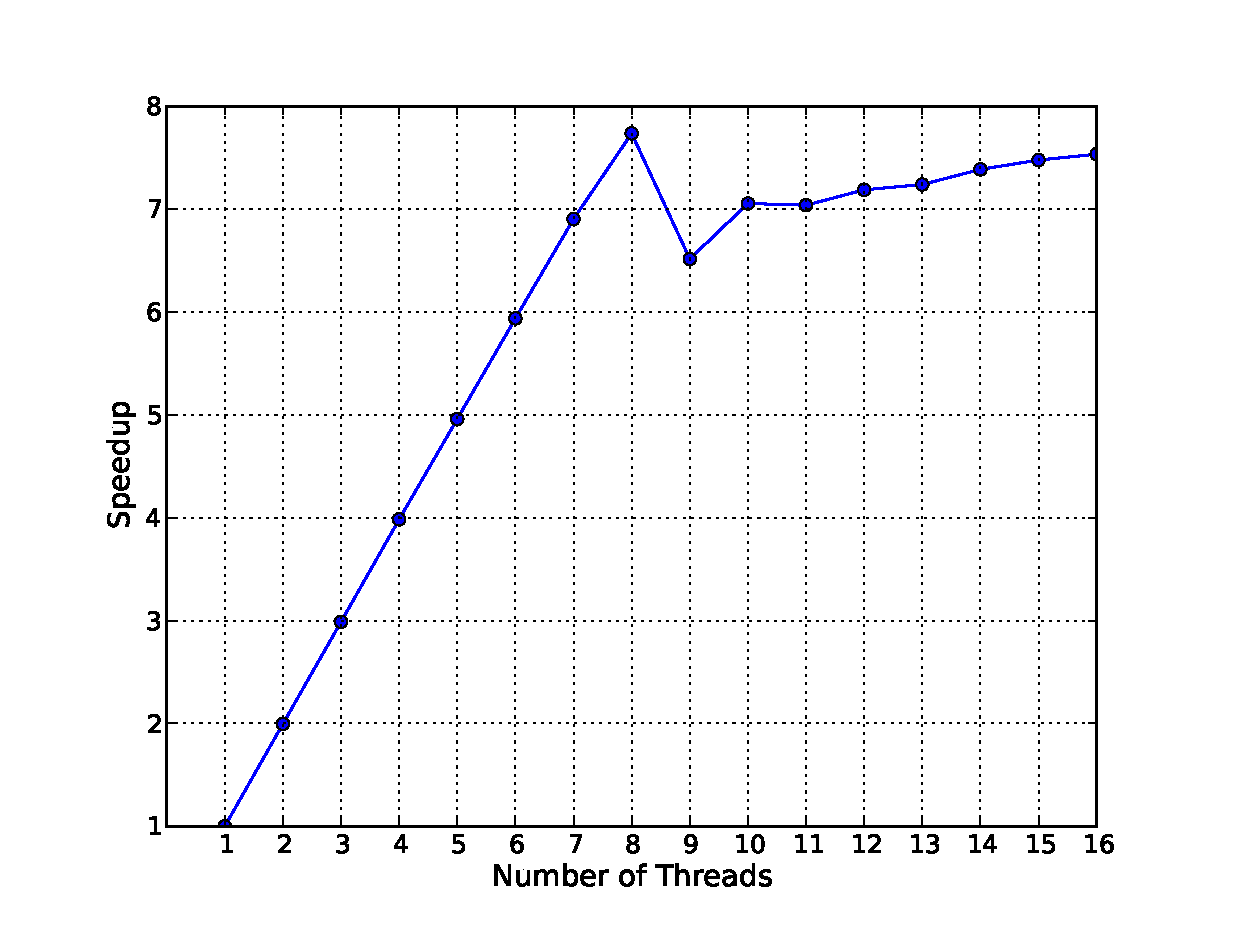
\includegraphics[width=3.8in]{coinspeedup.eps}
            \caption{Speedup of CoinFlip for different number of threads}
            \label{fig:coinspeedup}
        \end{figure}

        \begin{figure}[htbp]
            \centering
            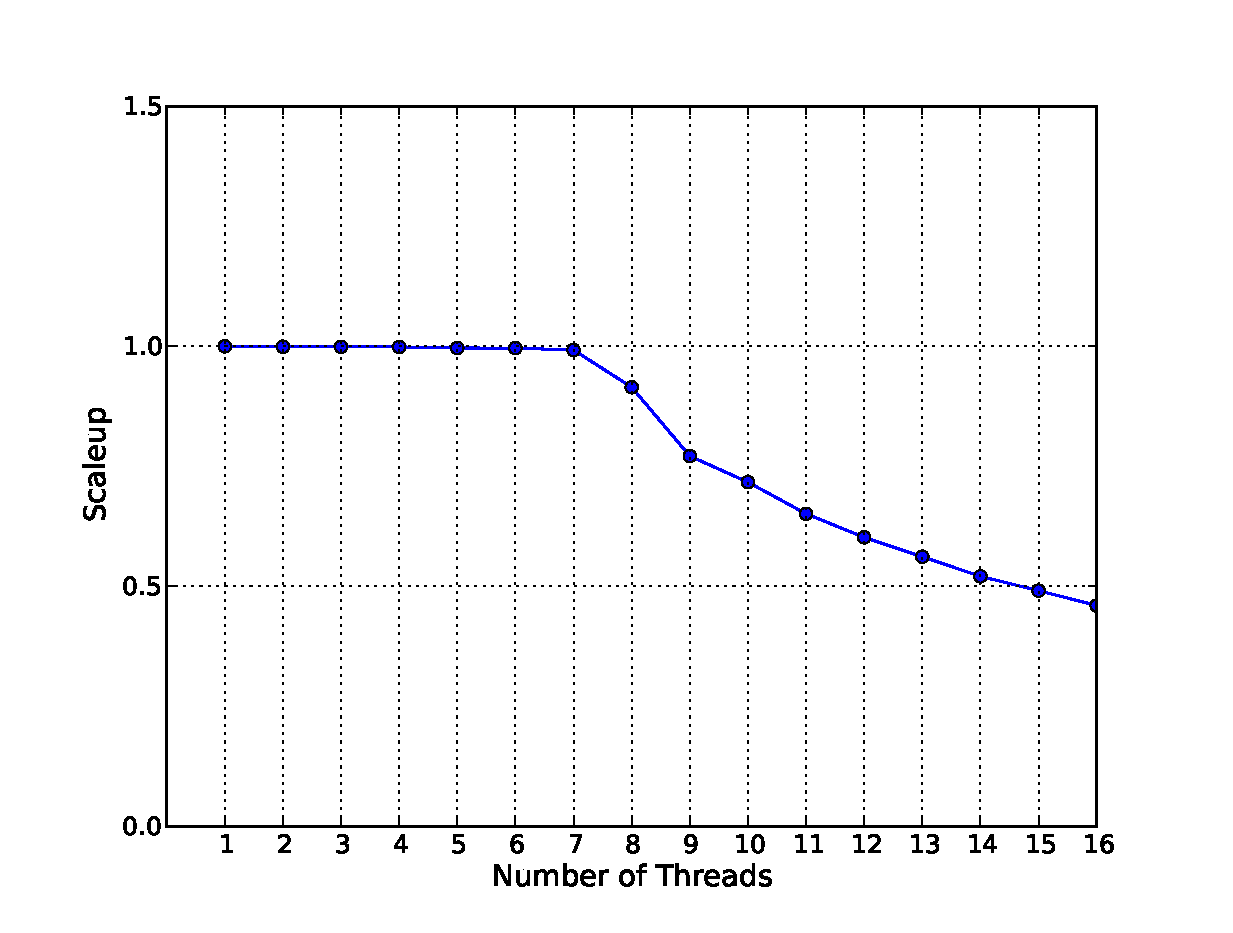
\includegraphics[width=3.8in]{coinscaleup.eps}
            \caption{Scaleup of CoinFlip for different number of threads}
            \label{fig:coinscaleup}
        \end{figure}
    \item \textbf{Algorithm (true) speedup/scaleup measures the scaling performance of the algorithm as a function of processing elements. In this case, from $1\dots8$. Characterize the algorithmic speedup/scaleup. If it is sub-linear, describe the potential sources of loss.}\\
        When the number of threads ranging from $1\dots8$, both the speedup and scaleup are almost linear. Only when the number of threads reaches $8$, the speedup/scaleup start to degrade. This is because I am running the program on a $8$-core machine, so the optimal number of threads is $8$. And the JVM is running a master thread, so the speedup and scaleup cannot keep linear when the number of slave threads reaches $8$.

    \item Why does the speedup not continue to increase past the number of cores? Does it degrade? Why?  \\
        As the processor has $8$ cores, it can have at most $8$ instructions executed per cycle. When I have $8$ threads running, the processor's execution resources have been well utilized. This is why the speedup does not continue to inscrease past the number of core. An obvious degradation can be observed when there are $9$ threads running. This is because of the latency of thread switching and startup cost.

\end{enumerate} 

\textbf{Design and run an experiment that measures the startup costs of this code.}
\begin{enumerate}
    \item \textbf{Describe your experiment. Why does it measure startup?}\\
        If we run the program with $0$ coin flippings, the time we get is the startup cost. This is because the threads are created and initialized but never actually put to work. 
    \item \textbf{Estimate startup cost. Justify your answer.}\\
        We run the program for $100, 200,$\\$ \dots, 500$ threads with $0$ iteration. The result is shown in Figure \ref{fig:coinstartup}.

        \begin{figure}[htbp]
            \centering
            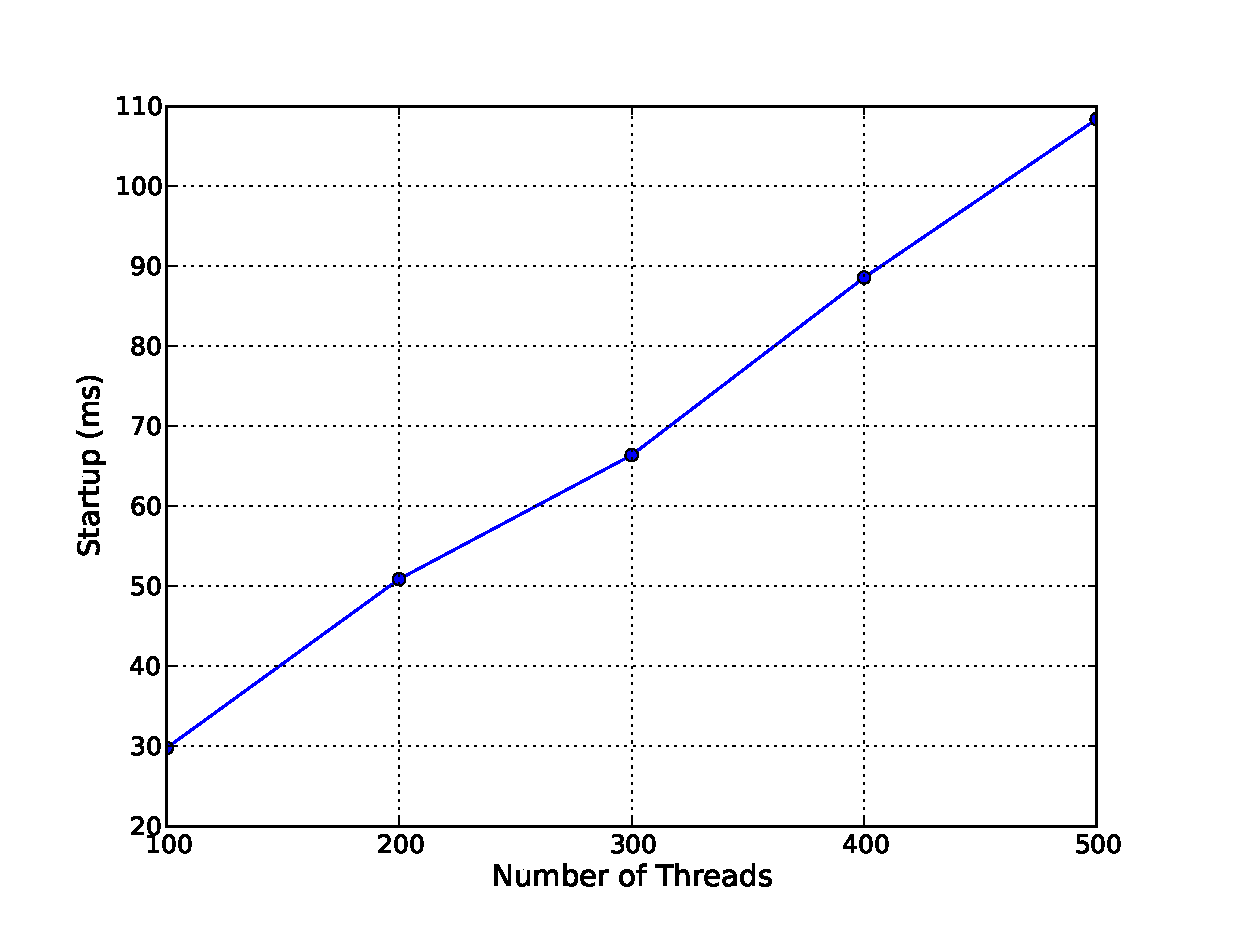
\includegraphics[width=3.8in]{coinstartup.eps}
            \caption{Startup of CoinFlip for different number of threads}
            \label{fig:coinstartup}
        \end{figure}
        From the figure, we estimate the startup cost $startup = 0.195 * \dot \#thread + 10.5$
    \item \textbf{Assuming that the startup costs are the serial portion of the code and the remaining time is the parallel portion of the code,what speedup would you expect to realize on 100 threads? 500 threads? 1000 threads? (Use Amdahl's law.)}\\
        Assume the $\#thread$ is $1$, the startup cost is about $10.7$ ms, and from part $1$ we know the running time is $9050$ ms, so we estimate the parallel portion to be $\frac{9050-10.7}{9050}=0.99$. Using Amdahl's law, the speedup is $\frac{1}{(1-P)+\frac{P}{S}}$.
        So with $P=0.99$, for $S=100$, the speedup is $50.25$. For $S=500$, the speedup is $83.47$, and for $S=1000$, the speedup is $90.99$.
\end{enumerate}
\newpage
\newpage
\section*{Problem 2}
\textbf{For reasonable parameters and for however many cores you have on the system, measure the scaleup and speedup of this program.}

\begin{enumerate}
    \item \textbf{Produce charts and interpret/describe the results. Is the speedup linear?}\\
        The program is run for $1, 2, \dots, 16$ threads with a key of $20$ bits long for speedup, and run for $1, 2, 4, 8, 16$ threads with $20, 21, 22, 23, 24$ bits long keys for scaleup.
        The speedup of the program is shown in Figure \ref{fig:desspeedup}, and the scaleup is shown in Figure \ref{fig:desscaleup}.
        \begin{figure}[htbp]
            \centering
            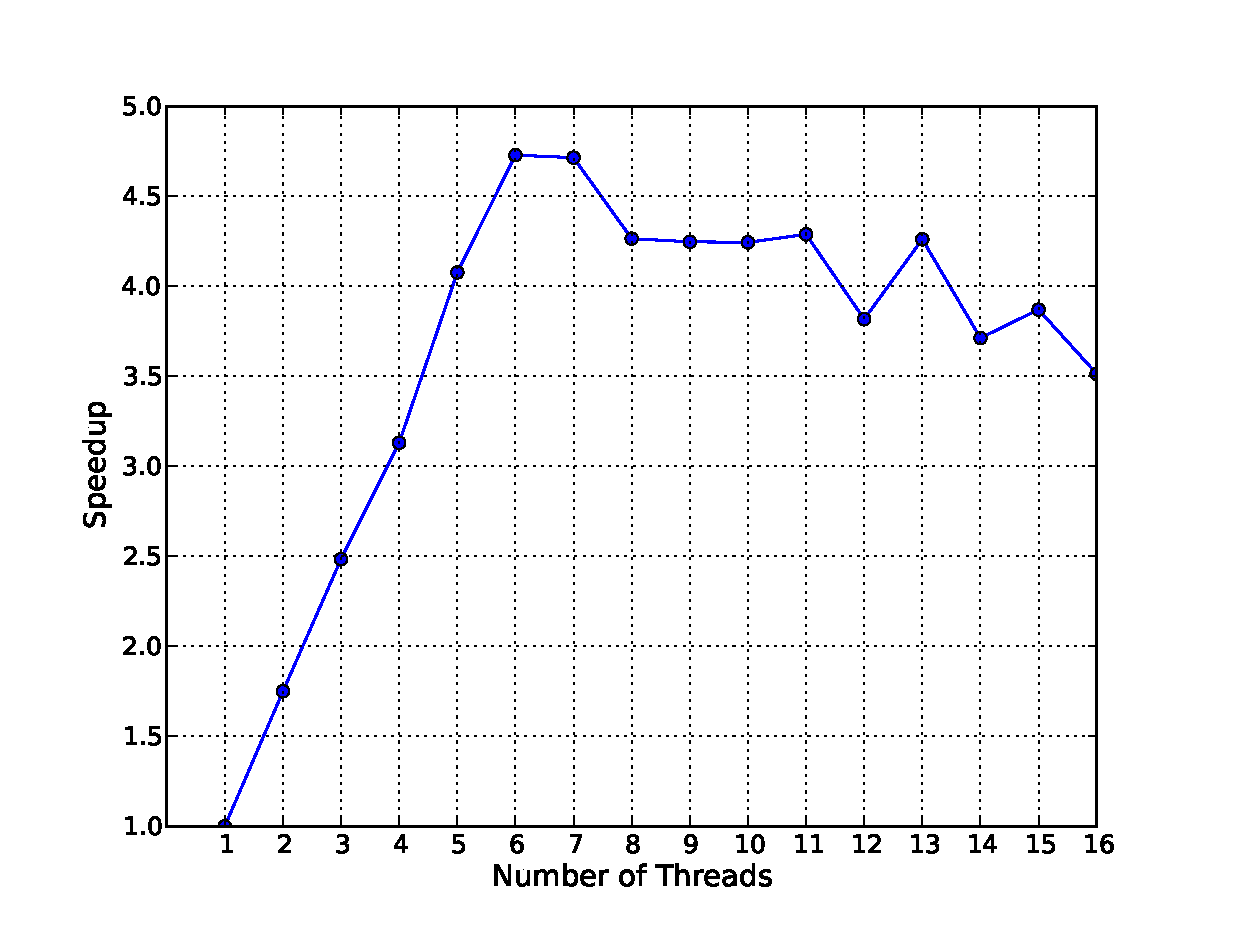
\includegraphics[width=3.8in]{desspeedup.eps}
            \caption{Speedup of BruteForceDES for different number of threads}
            \label{fig:desspeedup}
        \end{figure}

        \begin{figure}[htbp]
            \centering
            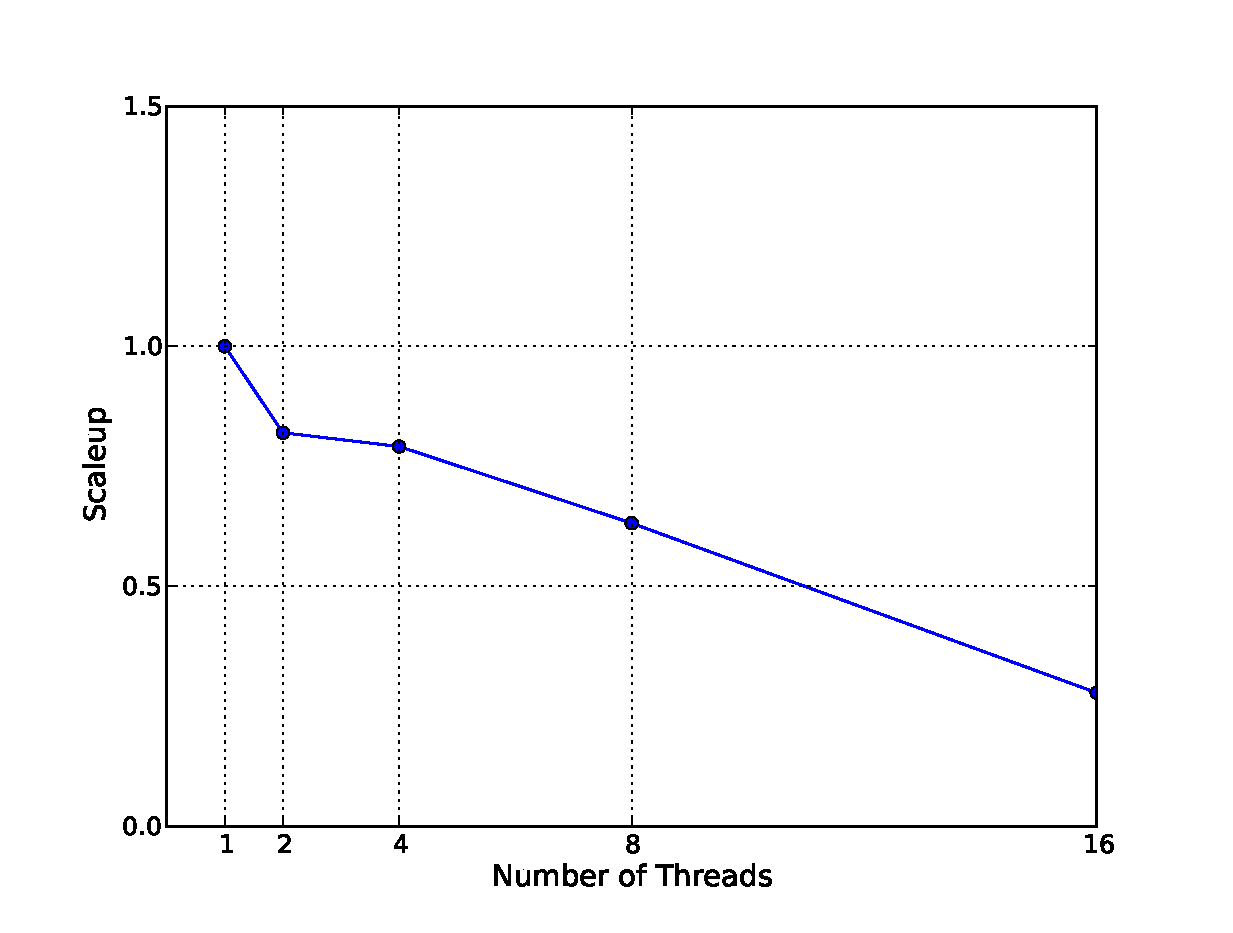
\includegraphics[width=3.8in]{desscaleup.eps}
            \caption{Scaleup of BruteForceDES for different number of threads}
            \label{fig:desscaleup}
        \end{figure}
        The speedup shows a near-linear increase when the thread number goes from $1$ to $6$, but it is not a linear speedup as doubling the number of threads doesn't double the speed. When the thread number reaches $7$, the increase gets down and finally starts to degrade.\\
        The scaleup keeps going down. And from $1$ thread to $2$ threads, the drop is particularly rapid. It is also not linear scaleup.
    \item \textbf{Why do you think that your scaleup/speedup are less than linear? What are the causes for the loss of parallel efficiency?}\\
        As I use a separate \texttt{SealedObject} for each of the working threads, and I make every thread create its own \texttt{SealedDES} object to do the decryption, there should be no shared resources between the threads. And as I have less threads than cores, there should be not much context switching overhead to affect the speedup. And the job is divided evenly among all the threads, there is no skew problem. So the cause of the sublinear speedup/scaleup is the startup
        cost. The portion of operations that cannot be run in parallel has lower the speedup increase, and because of Amdahl's law the speedup and scaleup are sublinear.
    \item \textbf{Extrapolating from your scaleup analysis, how long would it take to brute force a 56 bit DES key on a machine with 64 cores? Explain your answer.}\\
        Assume the scaleup to be $S_{64}$ with $64$ threads. We suppose for $1$ thread and $20$-bits key, the running time is $T_{1}$; for $64$ threads and $26$-bits key, the running time is $T_{64}$. Here we have $S_{64}=T_{1}/T_{64}$. From previous analysis, $T_{1}=10051ms$. To brute force a $56$ bit DES key, the time should be
        $T=2^{30}T_{64}=2^{30}\frac{T_{1}}{S_{64}}=\frac{2^{31}}{S_{64}}s$. If we have a linear scaleup, it will take about $2^{31}s$, which is about $68$ years to brute force the 56 bit key. Extrapolating our scaleup analysis,
        $S_{64}$ will be a much smaller number, so the time to brute force a $56$ bit key on a $64$ core machine will be very large.
\end{enumerate}



\end{document}




































